%
%
%          Doc ...... UMKC Dissertation, v 1.0
%          Style .... APA 7
%          Date ..... May 23rd, 2025
%          Author ... Oleksandr Valchyshen, 
%                     avpfc@umkc.edu, valchyshen@gmail.com
%

\documentclass[12pt]{article}

% --- Bibliography, APA 7 style ------------------------------------------+
\usepackage[style=apa,language=american,maxnames=2,minnames=2,sortcites=true]{biblatex} % maxcitenames=2
\DeclareLanguageMapping{american}{american-apa}
\addbibresource{ref.bib}

% --- Text look: font family, size, etc -----------------------------------+
%\usepackage{mathptmx} % <----------------------------- Uses New Times font
\usepackage{lmodern}   % <--------------------------- Uses Latin Modern font
\fontsize{12}{1} \selectfont % <------------------------- Sets the font size 
\usepackage{setspace}  % <----------------------------------------- Text spacing
\doublespacing %\singlespacing
%% set par indent
%\usepackage{indentfirst}
\setlength{\parindent}{5ex} % <----------------------------------- Text intend

% --- Set the page margins as required -----------------------------------------+
% Page Margins: no less than 1.25in for left, and 1in for right, top, bottom
\usepackage[left=1.25in,right=1in,top=1in,bottom=1.25in]{geometry}
\usepackage{lscape} % <---------------------------------- For landscape pages
\usepackage{pdflscape}
\usepackage{graphicx} % <--------------------- Required for inserting images
\usepackage[linktocpage=true]{hyperref}
\hypersetup{
    colorlinks  = {false},
    linkcolor   = {blue},
    filecolor   = {magenta},      
    urlcolor    = {cyan},
    pdftitle    = {Dissertation by Oleksandr Valchyshen},
    pdfpagemode = {FullScreen},
}
\usepackage{varioref}
\usepackage[utf8]{inputenc}
% For rotating figures, tables, etc.
%  including their captions
\usepackage{rotating}

% --- Folders --------------------------------------------------------------+
\newcommand{\folder}{./Sections} % <------------ the forlder for all chapters 
\newcommand{\plotsfolder}{./Plots} % <------------------ the folder for plots
\newcommand{\imagesfolder}{./Images} % <--------------- the folder for images
\usepackage{setspace}\doublespacing % <------- Double-spacing the main text 
\expandafter\def\expandafter\quote  % <------ Single-spacing the quotes used
\expandafter{\quote\small\singlespacing}
\usepackage{endnotes,chngcntr}
\usepackage{booktabs}
\usepackage[perpage,symbol*]{footmisc}
\usepackage{titlesec}
\usepackage{soul}
\usepackage{afterpage}
\usepackage{stringstrings} % <--- https://www.ctan.org/pkg/stringstrings
\usepackage{tfrupee} % <------------------------- Symbol of Indian rupee
\usepackage{mfirstuc} % <--------- Capitalize titles: \capitalisewords{}
\usepackage{mwe}
\usepackage{mfirstuc}
%\usepackage{xcolor}
\usepackage[dvipsnames,svgnames,table]{xcolor}
\usepackage{etoolbox}
\usepackage{amsmath}
\usepackage{mathtools}
\usepackage{epsfig,graphics}
\usepackage[labelfont=bf,slc=off]{caption}
\usepackage{tikz}
\usepackage{pgfplots}\pgfplotsset{compat=1.18}
\usetikzlibrary{matrix,fit,arrows.meta,bending,positioning,arrows,shapes,
                shapes.multipart,automata,decorations.pathmorphing,calc}
                
% Tikz related function \gettikzxy
\makeatletter
\newcommand{\gettikzxy}[3]{%
  \tikz@scan@one@point\pgfutil@firstofone#1\relax
  \edef#2{\the\pgf@x}%
  \edef#3{\the\pgf@y}%
}
\makeatother
                  
% --- Acronyms/Abbreviations Section -------------------------------------------+
\usepackage{acro}
% --- List of Acronyms/Abbreviations ---------------- %
\DeclareAcronym{umkc}{
  short=UMKC,
  long=University of Missouri-Kansas City,
}
\DeclareAcronym{afit}{
  short=AFIT,
  long=Association for Institutional Thought,
}
\DeclareAcronym{usd}{
  short=USD,
  long=U.S. Dollar,
}
\DeclareAcronym{reer}{
  short=REER,
  long=real effective exchange rate,
}
\DeclareAcronym{neer}{
  short=NEER,
  long=nominal effective exchange rate,
}
\DeclareAcronym{bis}{
  short=BIS,
  long=Bank for International Settlements,
} % List of acronyms, 2b updated
% acro dev page: https://github.com/cgnieder/acro
% acro manual:   https://mirror2.sandyriver.net/pub/ctan/macros/latex/contrib/acro/acro-manual.pdf

% --- Managing sections' titles ------------------------------------------------+
\usepackage{titlesec} % <- ...using this package to modify the section titles
% Level 1: the appearance of the CHAPTER...
\renewcommand\thesection{\arabic{section}}  % CHAPTER 1 [New Line] TITLE
\titleformat{\section}[display]             % each chapter has two lines...
    {\normalfont\fontfamily{lmr}\selectfont\filcenter}{\MakeUppercase{Chapter~\thesection}}{0pt}{}
\titlespacing*{\section}{0pt}{0pt}{24pt}    % 24pt after section/chapter
% Level 2: the appearance of the section...
\titleformat{\subsection}
    {\normalfont\fontfamily{lmr}\selectfont\bfseries\filcenter} 
    {\thesubsection}{1em}{}
\titlespacing*{\subsection}{0pt}{30pt}{6pt} % 30pt before, 6pt after subsection
% Level 3: the appearance of the subsection...
\titleformat{\subsubsection}
    {\normalfont\fontfamily{lmr}\selectfont\bfseries\itshape} 
    {\thesubsubsection}{1em}{}
\titlespacing*{\subsubsection}{0pt}{12pt}{6pt} % 30pt before, 6pt after subsection
% Level 4: the appearance of the subsubsection...
\setcounter{secnumdepth}{4}
\titleformat{\paragraph}
{\normalfont\fontfamily{lmr}\normalsize\itshape}{\theparagraph}{1em}{}
\titlespacing*{\paragraph}
{0pt}{3.25ex plus 1ex minus .2ex}{1.5ex plus .2ex}

% --- Capitalizing the titles of the respective sections -----------------------+
\renewcommand{\notesname}{\centering \MakeUppercase{Footnotes}}
\renewcommand{\contentsname}{\centering \MakeUppercase{Contents}}
\renewcommand{\refname}{\centering \MakeUppercase{References}}
\renewcommand{\listfigurename}{\centering \MakeUppercase{List of Illustrations}}
\renewcommand{\listtablename}{\centering \MakeUppercase{List of Tables}}
\usepackage[titles]{tocloft}      % <-- ...to modify ToC, LoF, and LoT
\renewcommand{\cftdotsep}{4}      % dots spacing
\renewcommand{\cftsecdotsep}{4}   % dots spacing for sections 
\renewcommand{\cftsubsecdotsep}{4}% dots spacing for subsections
\renewcommand{\cfttoctitlefont}{\hfill\Large} % ToC = Table of Contents
\renewcommand{\cftaftertoctitle}{\hfill}
\renewcommand{\cftloftitlefont}{\hfill\Large} % LoF = List of Figures
\renewcommand{\cftafterloftitle}{\hfill}
\renewcommand{\cftlottitlefont}{\hfill\Large} % LoT = List of Tables
\renewcommand{\cftafterlottitle}{\hfill}

% --- Endnotes -----------------------------------------------------------------+
% Reset endnote numbering every section
\counterwithin*{endnote}{section}
\counterwithin*{section}{part}
\let\latexsection\section
\makeatletter  %changes the catcode of @ to 11
\renewcommand\enoteheading{
    \setcounter{secnumdepth}{-2}
    \latexsection*{\notesname\markboth{NOTES}{}}
    \mbox{}\par\vskip-\baselineskip
    \let\@afterindentfalse\@afterindenttrue
}
\def\enotedivision#1#2{\@ifnextchar\enotedivision{}{#1{#2}}}
\makeatother    
\RenewDocumentCommand{\section}{som}{%
  \IfBooleanTF{#1}
  {\latexsection*{#3}%
    \setcounter{endnote}{0}%
    \addtoendnotes{%
      \noexpand\enotedivision{\noexpand\subsubsection*}
      {\unexpanded{#3}}}%
  }
  {\IfNoValueTF{#2}
    {\latexsection{#3}}
    {\latexsection[#2]{#3}}%
    \addtoendnotes{%
     \noexpand\enotedivision{\noexpand\subsubsection*}
     {\thesection. \unexpanded{#3}}}%
  }%
}
\let\footnote=\endnote
%--- ...end of Endnotes

% --- Making footnotes as hyperlinks -------------------------------------------+
\makeatletter
\def\@footnotecolor{red}
\define@key{Hyp}{footnotecolor}{%
 \HyColor@HyperrefColor{#1}\@footnotecolor%
}
\patchcmd{\@footnotemark}{\hyper@linkstart{link}}{\hyper@linkstart{footnote}}{}{}
\makeatother
\hypersetup{footnotecolor=red}

% --- Index Section ------------------------------------------------------------+
\usepackage{imakeidx} % <----------------------- Alphabetical Index, two columns
\makeindex[columns=2, title={\MakeUppercase{Index}}]

\usepackage{lipsum} % filler text

% New commands that deal with page numbering and ToC's line with Chapter word
\def\prelimsections{
    % Roman numbering of pages of preliminary sections
    \pagenumbering{roman} 
    \setcounter{page}{3} % <----- UMKC's req: the Abstract page # is [iii] in Roman
}
\def\mainsections{
    \newpage
    % Arabic numbering for pages of main text: chapters, sections, subsections
    \pagenumbering{arabic}
    % sets the page counter at #1
    \setcounter{page}{1}
    % adds Chapter word into Table of Contents
    \addtocontents{toc}{\vspace{10pt}\protect\noindent% 
        Chapter \vspace{-4pt}\par} 
}
 % <--- sets up all needed packages

\begin{document} % === START OF THE DOCUMENT ==============================

% PART that initiates the project
%
%
%         MY INFO -------------------------
%      
%         author's name, thesis title, 
%         committee details, etc.
%         ---------------------------------
%      

% My thesis title: "[XXXXXXX Title page has title centered and in all capital letters and this is a long title so double-space it XXXXXXXXXXXXX XXXXXXXXX XXXX XXXXXXX XXXX XXXXXX]"  
% Change the text inside these brackets {...} in the next line
\newcommand{\MyThesisTitle}{[XXXXXXX Title page has title centered and in all capital letters and this is a long title so double-space it XXXXXXXXXXXXX XXXXXXXXX XXXX XXXXXXX XXXX XXXXXX]}

% My full legal name: "[Full Legal Name]", for example: "Joanna Smith"  
% Change the text inside these brackets {...} in the next line
\newcommand{\MyName}{[Full Legal Name]}

% My school: "School of Graduate Studies"  
% Change the text inside these brackets {...} in the next line
\newcommand{\MyUMKCSchool}{School of Graduate Studies}

% My degree: [Official Name of Degree], for example "Doctor of Philosophy"  
% Change the text inside these brackets {...} in the next line
\newcommand{\MyDegree}{[Official Name of Degree]}

% My degree is to be earned in the year of: "2025"  
% Change the text inside these brackets {...} in the next line
\newcommand{\MyDegreeAwardYear}{[Year Degree Earned]}

% Since I am in the I-PhD program, my co-discipline, "Social 
% Science Consorcium", is required to be named next to my core discipline, 
% "Economics".  
% Change the text inside these brackets {...} in the next line
\newcommand{\MyField}{[Official name of degree program] \par [and] \par [Official name of co-discipline if applicable]}

% The type of my work is: "Dissertation"  
% If it's "Thesis", then...
% ...change the text inside these brackets {...} in the next line
\newcommand{\ThesisOrDissertation}{[Thesis or Dissertation]}

% My previous degree, for example: "M.S., Oxford College, 2022"
% Change the text inside these brackets {...} in the next line
\newcommand{\MyPrevDegree}{[Initials of Previous Degree Earned, University Name, Graduation Year] \par [Type Additional Degrees Earned If Applicable]}

% My supervisory committee consists of five members:
%
%     Name         Department      Status
%     ----         ----------      ------
%     Kathy Stuart Economics       Committee Chair
%     Tom Muller   Economics       Member 1
%     Tod Hills    Economics       Member 2
%     Chris Black  Economics       Member 3
%     Mia Cooper   Social Science  Member 4
%
% Change the text inside these brackets {...} in the next line

\newcommand{\MyChair}{Kathy Stuart}
\newcommand{\MyChairDept}{Department of Economics}

\newcommand{\MyComOne}{Tom Muller}
\newcommand{\MyComOneD}{Department of Economics}

\newcommand{\MyComTwo}{Tod Hills}
\newcommand{\MyComTwoD}{Department of Economics}

\newcommand{\MyComThree}{Chris Black}
\newcommand{\MyComThreeD}{Department of Economics}

\newcommand{\MyComFour}{Mia Cooper}
\newcommand{\MyComFourD}{Department of Sociology}

 % <---------------- Key details of PhD thesis
\begin{center}
\thispagestyle{empty} % <---- this page is not numbered

\setlength{\baselineskip}{28pt}
\vspace*{.6in}

% Title of the Dissertation
\Large{
  \MakeUppercase{\MyThesisTitle}
} 
\normalsize

\setlength{\baselineskip}{13pt}
\vspace*{1.25in}

A \MakeUppercase{\ThesisOrDissertation}\\
IN\\
\vspace{0.1in}
\MyField\\
\vspace{0.5in}

Presented to the Faculty of the University\\
of Missouri--Kansas City in partial fulfillment of\\
the requirements for the degree

\vspace{0.5in}
\MakeUppercase{\MyDegree}
\vspace{0.95in}

by\\
\vspace{0.1in}
\MakeUppercase{\MyName} \\
\vspace{0.15in} 
\MyPrevDegree \\

\vspace{1.5in}
Kansas City, Missouri\\
\MyDegreeAwardYear

\end{center}\newpage
 % <----------------- Title page
\thispagestyle{empty}  % <---- this page is not numbered
\vspace*{7in}
\doublespacing

\begin{center}
\copyright \hspace{0.02in} \MyDegreeAwardYear \\
\MakeUppercase{\MyName} \\
\MakeUppercase{All Rights Reserved} 
\end{center}\newpage
 % <------------- Copyright page
\prelimsections % <--- command from tools.tex
\begin{center}
\vspace*{0.01in}
\large{\MakeUppercase{\MyThesisTitle}}\\
\vspace{24pt}
\normalsize{
  \MyName, Candidate for the \MyDegree\ Degree\\
  University of Missouri--Kansas City, \MyDegreeAwardYear\\
  \vspace{24pt}
  \MakeUppercase{Abstract}
  \vspace{12pt}
}
\end{center}
\addcontentsline{toc}{section}{ABSTRACT} % <--- the name 'ABSTRACT' will appear in the Table of Contents, as a chapter

\doublespacing

%%%   Place the text of your abstract below, ... 
%%%   instead of line 20

\lipsum[1-2] % <--- text fill, random text
 % <-------------- Abstract page
\newpage
\section*{\MakeUppercase{Approval Page}}

\setlength{\baselineskip}{24pt}
The faculty listed below, appointed by the Dean of the \MyUMKCSchool,
 have examined a \MakeLowercase{\ThesisOrDissertation}\ titled
``\MyThesisTitle,''~presented by \MyName, candidate
for the \MyDegree degree, and  certify that in
their opinion it is worthy of acceptance.

\vspace{0.5in}
\setlength{\baselineskip}{5pt}

\begin{center}
\underline{Supervisory Committee} \\

\vspace{0.25in}
\MyChair, Ph.D., Committee Chair \\
\MyChairDept \\

\vspace{0.25in}
\MyComOne, Ph.D.\\
\MyComOneD \\

\vspace{0.25in}
\MyComTwo, Ph.D.\\
\MyComTwoD \\

\vspace{0.25in}
\MyComThree, Ph.D.\\
\MyComThreeD \\

\vspace{0.25in}
\MyComFour, Ph.D.\\
\MyComFourD \\

\end{center} \doublespacing  % <-------------- Approval page
\newpage

% Table of Contents + making TOC not in bold font
{\let\bfseries\mdseries \tableofcontents} \newpage

% List of Figures/Illustrations
\listoffigures 
\addtocontents{lof}{{~Figure}~\hfill{Page}\par} % <- inserting a line w/"Figure"
\addcontentsline{toc}{section}{\MakeUppercase{List of Illustrations}}
\newpage

% List of Tables
\listoftables
\addtocontents{lot}{{~Table}~\hfill{Page}\par} % <- inserting a line w/ "Table"
\addcontentsline{toc}{section}{\MakeUppercase{List of Tables}}
\newpage 

% List of Acronyms/Abbreviations
\printacronyms[pages={display=all,seq/use=false},name=\MakeUppercase{List of Acronyms}]
%\addtocontents{loa}{{~Acronym}~\hfill{Page(s)}\par} % <- inserting a line w/ "Acronym"
\addcontentsline{toc}{section}{\MakeUppercase{List of Acronyms}}
\newpage % <------------------- Table of Contents
\section*{\MakeUppercase{Acknowledgments}}
\addcontentsline{toc}{section}{\MakeUppercase{Acknowledgments}}

%%%   Place the text of your acknowledgments below, ... 
%%%   instead of lines 7-9

I am grateful to the professors of my supervisor committee from the economics and sociology departments at \ac{umkc}. 

\lipsum[1-2] % <--- text fill, random text

\section*{\MakeUppercase{Preface}}
\addcontentsline{toc}{section}{\MakeUppercase{Preface}}

%%
%%   If your work (dissertation/thesis) has a Preface,
%%   place its text below instead of lines 9-26
%% 

Hello, world! This is an example of a dissertation formatted according to the guidelines of \ac{umkc}.\footnote{An example of footnote.} Below is an example of image placed in Figure~\ref{fig:image1}, p.~\pageref{fig:image1}.

\begin{figure}[!ht]
    \vspace{.4in}
    % The figure's caption and notes lines are centered, 75% of page width 
    \captionsetup{width=.75\linewidth,labelfont=bf}
    \caption{Example of an image sized to 75\% of the page width}
    \vspace{.2in}
    \centering
    % The plot is 75% of its width
    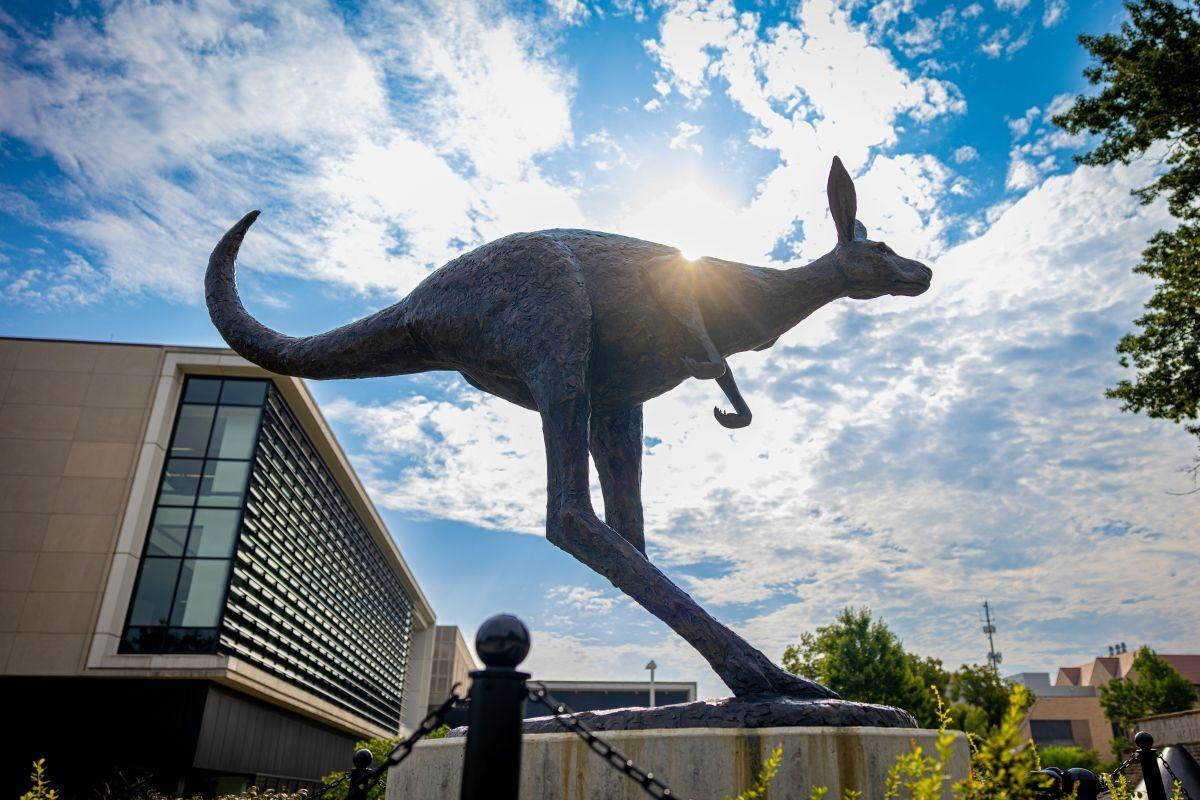
\includegraphics[width=.75\linewidth]{Images/UMKC_Roos.jpg}
    \vspace{.2in}
    \caption*{Note: some notes. \par\vspace{.15in} Source: \ac{umkc}, \url{https://www.umkc.edu/}}
    \vspace{.2in}
    \label{fig:image1}
\end{figure}

\lipsum[1-3] % text fill, random text % <--- put % before \input{...} if there is no Preface

% PART that is the core of the project --- Author's CHAPTERS
\mainsections % <--- command from tools.tex
%
%
%        CHAPTER 1
%        SOME CHAPTER TITLE
%
%

\newpage
\section{\MakeUppercase{Some Chapter Title}}\label{sec:ch1}

\subsection{Example of level 2 section \& citations, plots}

This is an example of text within a Chapter~\ref{sec:ch1}.\footnote{This is an example of a footnote made in Chapter~\ref{sec:ch1}.} The following paragraph shows an example of a quote with a citation.

Thus, in the 1930s, \citeauthor{book1} wrote his major work: the book titled the \citetitle{book1}. Through the content of the book, the author produced a revolution in the thinking about the economic organization of modern-day societies. In particular, he started the book with a preface by saying:

\begin{quote}
    This book is chiefly addressed to my fellow economists. I hope it will be intelligible to others. But its main purpose is to deal with difficult questions of theory, and only in the second place with the applications of this theory to practice.~\parencite[p.~v]{book1}
\end{quote}

Another example of citations is this. In \textcite{article1}, the author criticizes a theoretical approach in economics that equates international trade in goods and in financial instruments. Hence, the article's title \citetitle{article1} gives the general idea of the author's argument.

A journal paper reference is like this. In \textcite{article2}, the author explains how central banks set interest rates. This paper concludes: ``the ability to set interest rates is most assuredly a matter of \textit{political} economy'' (emphasis original). See Figure~\ref{} from Appendix~\ref{apx:A}.

Also, the citation of a source with several authors, in accordance with the APA~7 style, is: \textcite{wp1}, and a quote from it is: 

\begin{quote}
    In fact, \dots the modalities of hawala transmission are \textit{similar} to other kinds of international payments, including those that go through formal banking systems. \parencite[p.~14, emphasis added]{wp1}
\end{quote}

The following example is of a plot.\footnote{Another example of a footnote made in Chapter~\ref{sec:ch1}.} See Figure~\ref{fig:plot1}, p.~\pageref{fig:plot1}. Also, a plot, if needed, can be presented at a landscape page as in Figure~\ref{fig:plot1_}, p.~\pageref{fig:plot1_}. 

There is another example of a plot depicting monthly data by \ac{bis}, such as Japan's \ac{neer}. It is in Figure~\ref{fig:plot2}, in the Appendix~\ref{apx:B} on p.~\pageref{fig:plot2}.

\begin{figure}[!ht]
    \vspace{.4in} % <--- some space between text and this figure's top
    % The figure's caption and notes lines are centered, 80% of page width 
    \captionsetup{width=.8\linewidth,labelfont=bf}
    \caption{Example of a plot, showing the U.S. map}
    \vspace{.2in}
    \centering
    % The plot is 100% of its width
    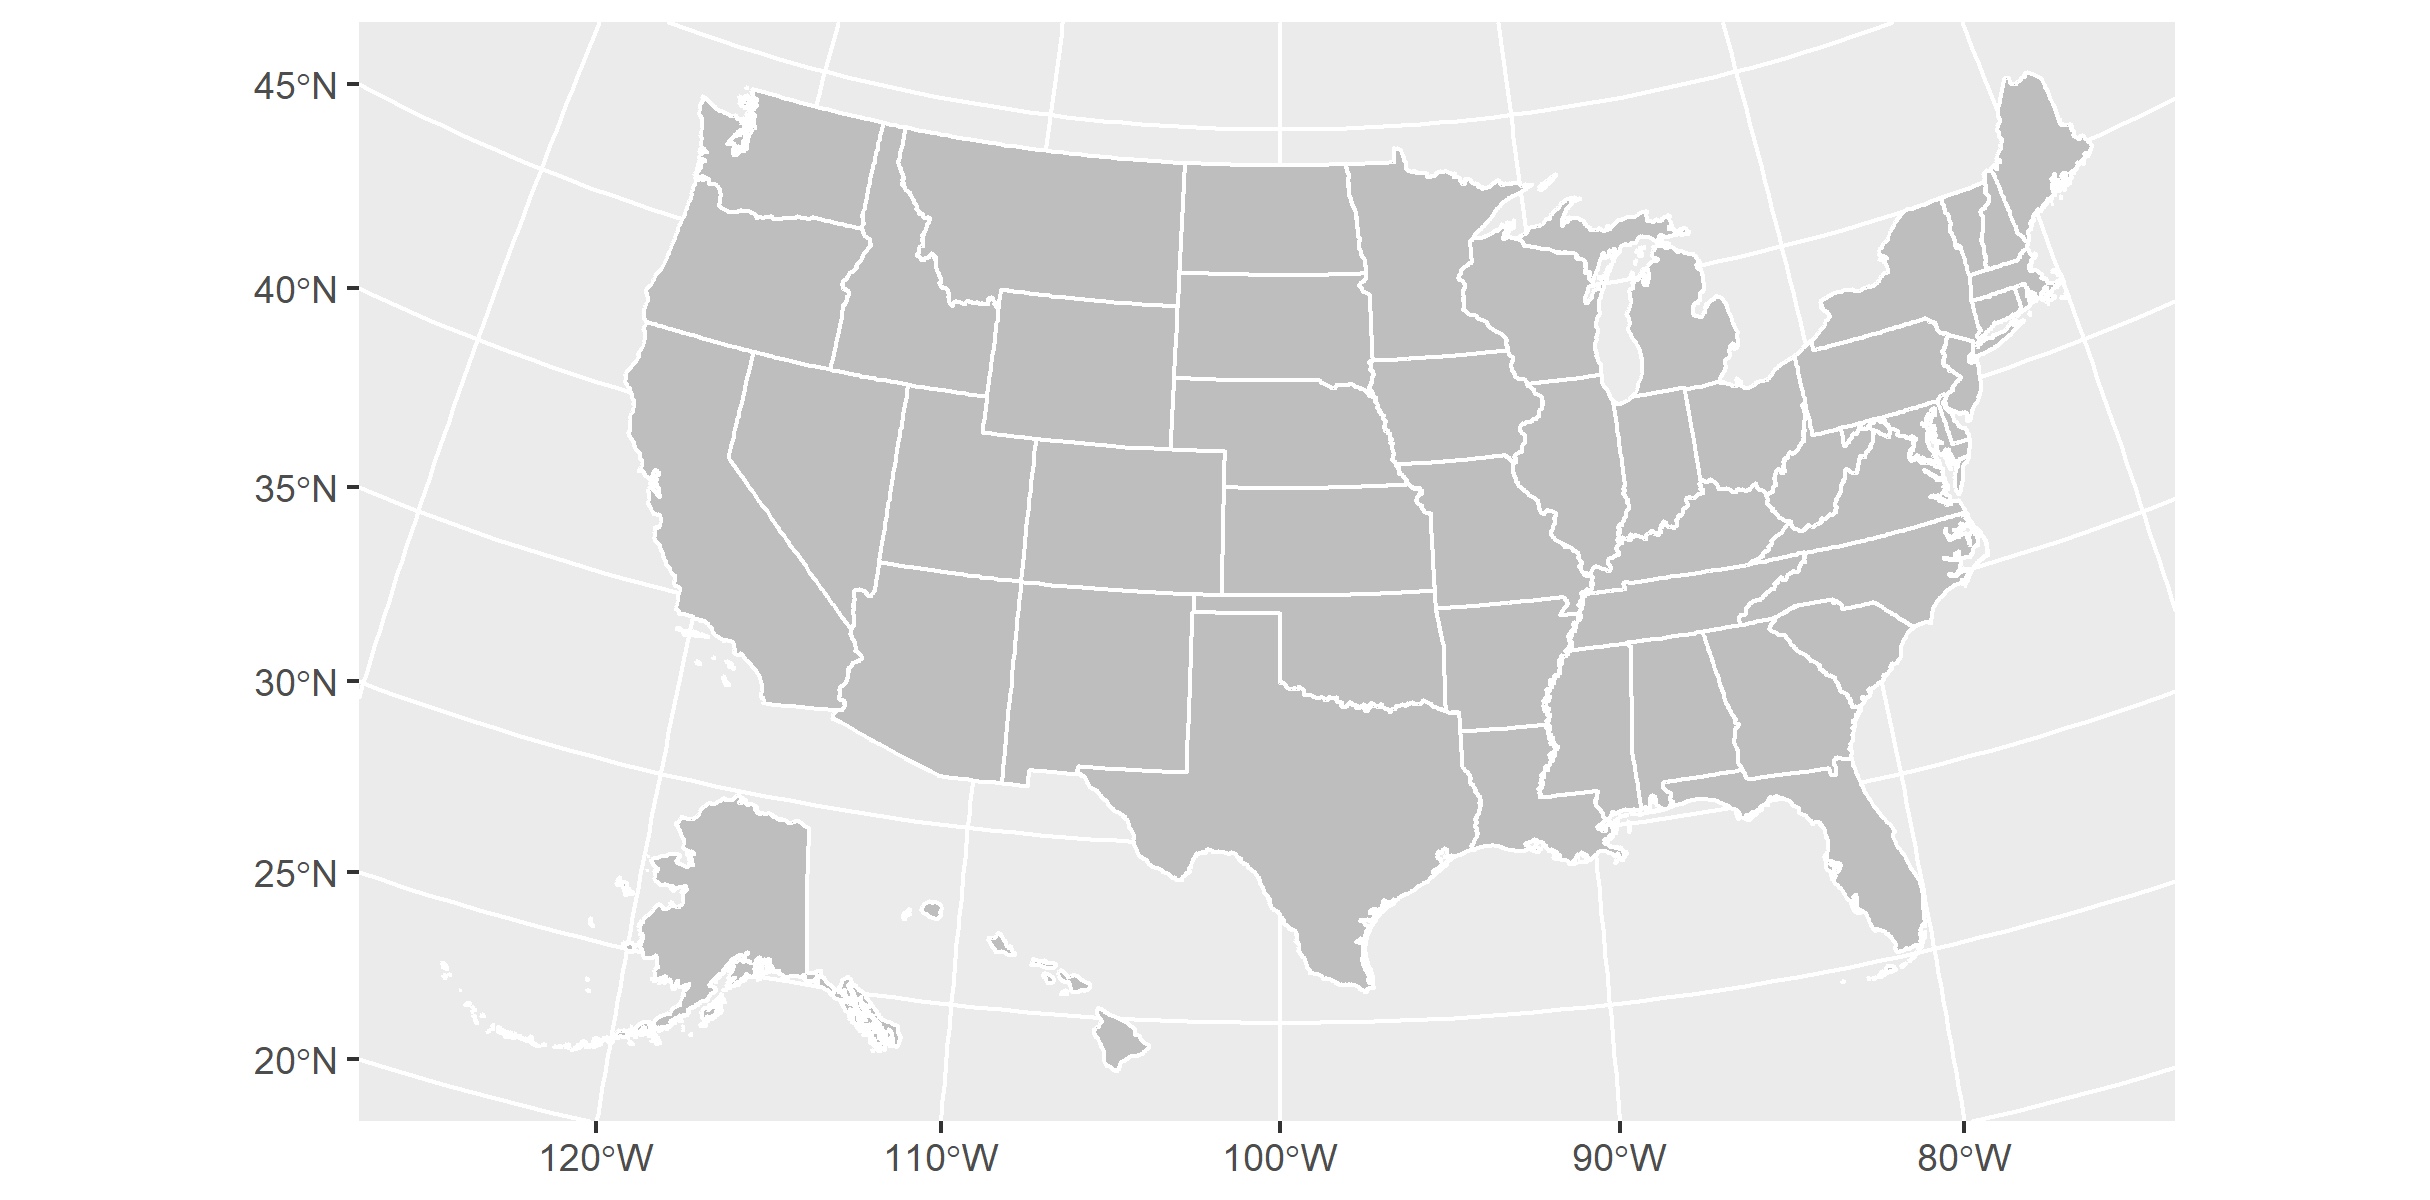
\includegraphics[width=1\linewidth]{Plots/Plot 1.png}
    \vspace{.2in}
    \caption*{Note: some notes. \par\vspace{.15in} Source: Some source here}
    \vspace{.2in} % <--- some space between text and this figure's bottom
    \label{fig:plot1}
\end{figure}

\begin{sidewaysfigure}[htbp]
    \vspace{.2in}
    % The figure's caption and notes lines are centered, 80% of page width 
    \captionsetup{width=1\linewidth,labelfont=bf}
    \caption{Example of a landscape plot, showing the U.S. map}
    \vspace{.2in}
    \centering
    % The plot is 100% of its width
    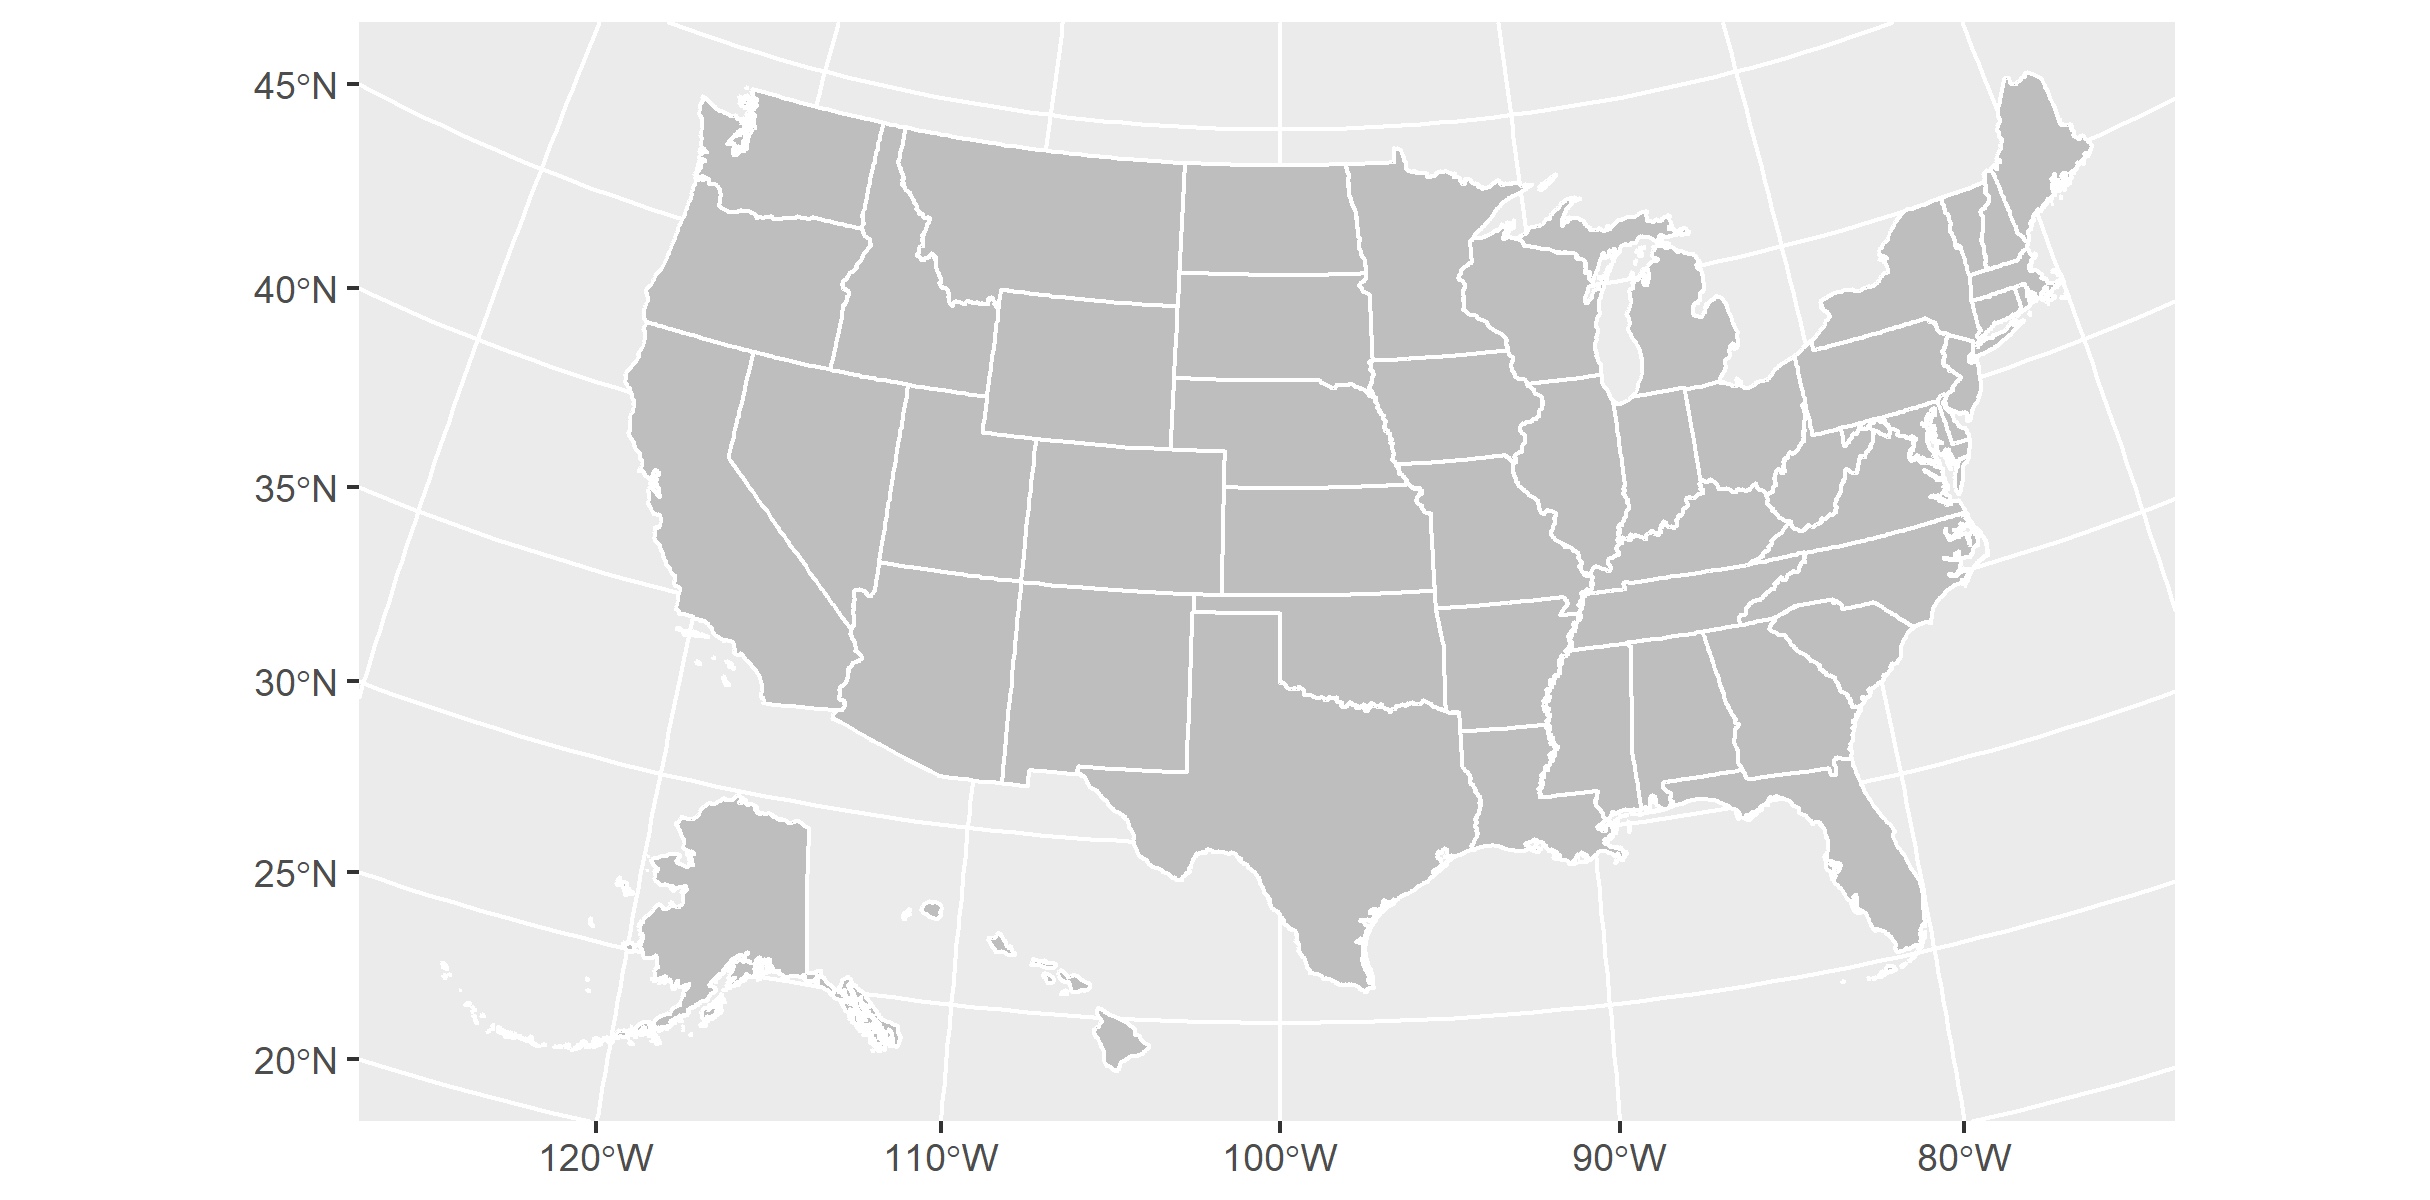
\includegraphics[width=1\linewidth]{Plots/Plot 1.png}
    \vspace{.2in}
    \caption*{Note: some notes. \par\vspace{.15in} Source: Some source here}
    \vspace{.2in}
    \label{fig:plot1_}
\end{sidewaysfigure}

\subsubsection{Example of level 3 section \& \emph{TiKz} plot}

A simple \emph{TikZ} plot is shown in Figure~\ref{fig:tikz1}, p.~\pageref{fig:tikz1}. The \texttt{tikz} package allows for the construction of quite elaborate plots. An example of such plot is provided in Appendix~\ref{apx:B}.

\begin{figure}[!ht]
    \vspace{.4in}
    % The figure's caption and notes lines are centered, 75% of page width 
    \captionsetup{width=.5\linewidth,labelfont=bf}
    \caption{Example of a simple \emph{TiKz} plot}
    \vspace{.2in}
    \centering
    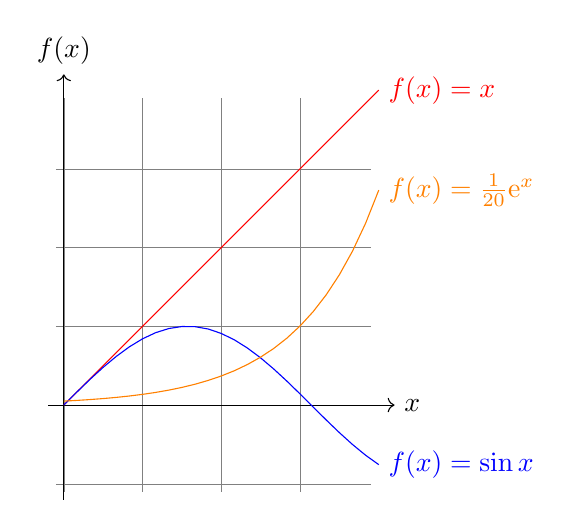
\begin{tikzpicture}[domain=0:4]
        \draw[very thin,color=gray] (-0.1,-1.1) grid (3.9,3.9);
        \draw[->] (-0.2,0) -- (4.2,0) node[right] {$x$};
        \draw[->] (0,-1.2) -- (0,4.2) node[above] {$f(x)$};
        \draw[color=red]    plot (\x,\x)             node[right] {$f(x) =x$};
        % \x r means to convert '\x' from degrees to _r_adians:
        \draw[color=blue]   plot (\x,{sin(\x r)})    node[right] {$f(x) = \sin x$};
        \draw[color=orange] plot (\x,{0.05*exp(\x)}) node[right] {$f(x) = \frac{1}{20} \mathrm e^x$};
    \end{tikzpicture}
    \vspace{.2in}
    \caption*{Note: some notes. \par\vspace{.15in} Source: \url{https://tikz.dev/tikz-plots}}
    \vspace{.2in}
    \label{fig:tikz1}
\end{figure}

\paragraph*{Example of level 4 section}
\lipsum[1-2]
 % <-------------- CHAPTER 1
%
%
%        CHAPTER 2
%        SOME CHAPTER TITLE
%
%

\newpage
\section{\MakeUppercase{Some Chapter Title}}\label{sec:ch2}

\subsection{Example of level 2 section \& tables}

Below are two table examples: (1) a \emph{\LaTeX} table, and {2) a \emph{TikZ} table.\footnote{Example of a footnote in Chapter~\ref{sec:ch2}.} The former is shown in Figure~\ref{tab:tbl1} below, while the latter is in Figure~\ref{tab:tbl2} on p.~\pageref{tab:tbl2}. Another example is of the landscape table, which is constructed by using \emph{TikZ} coding, see Figure~\ref{tab:tbl3} on p.~\pageref{tab:tbl3}.  

\begin{table}[!ht]
    \vspace{.4in}
    \captionsetup{width=.5\linewidth,labelfont=bf}
    \caption{Example of a \emph{\LaTeX} table}
    \vspace{.2in}
    \centering
    \begin{tabular}{lrr}
        \toprule
        Item   & Quantity & Price\textsuperscript{a}  \\
        \midrule
        Apple  & 5        & \$0.99 \\
        Orange & 3        & \$0.75 \\
        Banana & 4        & \$0.50 \\
        \bottomrule
    \end{tabular}
    \vspace{.2in}
    \caption*{Note: \textsuperscript{a}Price is provided in the \ac{usd}. \par\vspace{.15in} Source: some source}
    \label{tab:tbl1}
    \vspace{.2in}
\end{table}

\lipsum[1]

\begin{table}[!ht]
    \vspace{.4in}
    \captionsetup{width=.9\linewidth,labelfont=bf}
    \caption{Example of a \emph{TikZ} table}
    \vspace{.2in}
    \centering
    
\begin{tikzpicture}
    % Individual A -----------------------------------------------------
        \matrix [matrix anchor=north, matrix of nodes, nodes in empty cells,
             nodes = {text width=2.3in, minimum height=.2in, align=left},
             column sep=1em,
             row 2/.style={align=center, font=\bfseries},
            ] (n) at (8,4) 
        {
         & \\
        Assets & Liabilities \& Net Worth \\
        Financial Assets ($FA$) & Financial Liabilities ($FL$) \\
        Non-Financial Assets ($NFA$) & Net Worth ($NW$) \\
         };
        \node[fit=(n-1-1)(n-1-2)]%
        {\textit{\MakeUppercase{Balance sheet}\textsuperscript{a}}};
        \draw[thin]  (n-2-2.south -| n.west) -- (n-2-2.south -| n.east);
        \draw[thin]  (n-1-1.south east) -- (n-4-1.south east);
    \end{tikzpicture}
    \vspace{.2in}
    \caption*{Note: \textsuperscript{a}Denominated in the \ac{usd}. \par\vspace{.15in} Source: some source}
    \label{tab:tbl2}
    \vspace{.2in}
\end{table}

\lipsum[2]

\begin{sidewaystable}[htbp]
    \vspace{.4in}
    \captionsetup{width=1\linewidth,labelfont=bf}
    \caption{Example of a landscape \emph{TikZ} table}
    \vspace{.2in}
    \centering
    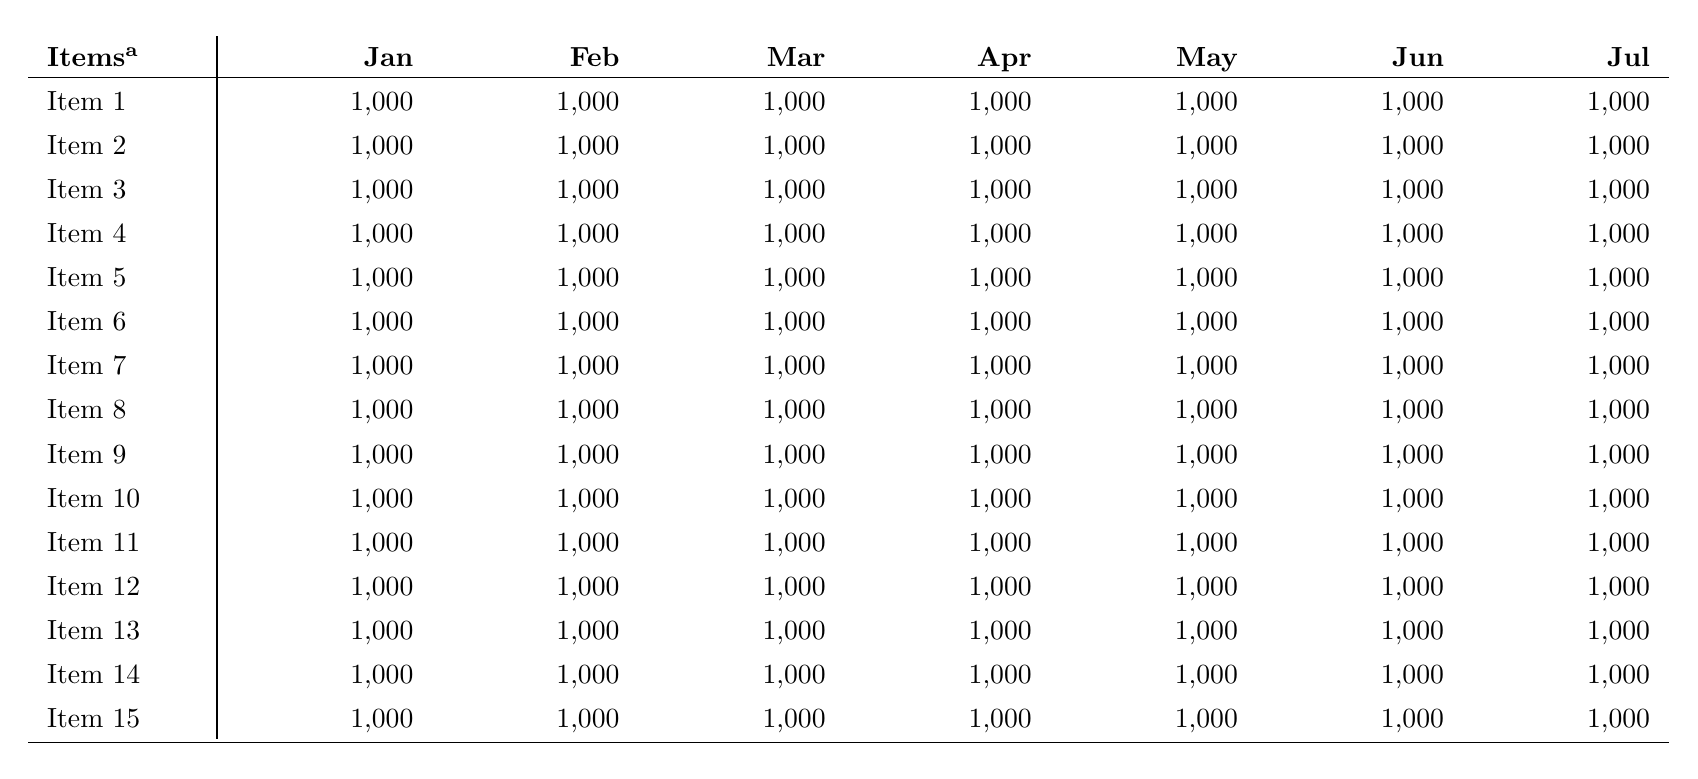
\begin{tikzpicture}
    % Individual A -----------------------------------------------------
        \matrix [matrix anchor=north, matrix of nodes, nodes in empty cells,
             nodes = {text width=.8in, minimum height=.2in, align=right},
             column sep=1em,
             row 1/.style={font=\bfseries},
             column 1/.style={nodes={align=left}}
            ] (n) %at (8,4) 
        {
        Items\textsuperscript{a}     
                    & Jan   & Feb   & Mar   & Apr   & May   & Jun   & Jul   \\
        Item 1      & 1,000 & 1,000 & 1,000 & 1,000 & 1,000 & 1,000 & 1,000 \\
        Item 2      & 1,000 & 1,000 & 1,000 & 1,000 & 1,000 & 1,000 & 1,000 \\
        Item 3      & 1,000 & 1,000 & 1,000 & 1,000 & 1,000 & 1,000 & 1,000 \\
        Item 4      & 1,000 & 1,000 & 1,000 & 1,000 & 1,000 & 1,000 & 1,000 \\
        Item 5      & 1,000 & 1,000 & 1,000 & 1,000 & 1,000 & 1,000 & 1,000 \\
        Item 6      & 1,000 & 1,000 & 1,000 & 1,000 & 1,000 & 1,000 & 1,000 \\
        Item 7      & 1,000 & 1,000 & 1,000 & 1,000 & 1,000 & 1,000 & 1,000 \\
        Item 8      & 1,000 & 1,000 & 1,000 & 1,000 & 1,000 & 1,000 & 1,000 \\
        Item 9      & 1,000 & 1,000 & 1,000 & 1,000 & 1,000 & 1,000 & 1,000 \\
        Item 10     & 1,000 & 1,000 & 1,000 & 1,000 & 1,000 & 1,000 & 1,000 \\
        Item 11     & 1,000 & 1,000 & 1,000 & 1,000 & 1,000 & 1,000 & 1,000 \\
        Item 12     & 1,000 & 1,000 & 1,000 & 1,000 & 1,000 & 1,000 & 1,000 \\
        Item 13     & 1,000 & 1,000 & 1,000 & 1,000 & 1,000 & 1,000 & 1,000 \\
        Item 14     & 1,000 & 1,000 & 1,000 & 1,000 & 1,000 & 1,000 & 1,000 \\
        Item 15     & 1,000 & 1,000 & 1,000 & 1,000 & 1,000 & 1,000 & 1,000 \\
        };
        \draw[thin]  (n-1-2.south -| n.west) -- (n-1-2.south -| n.east);
        \draw[thin]  (n-1-1.north east) -- (n-16-1.south east);
        \draw[thin]  (n-16-2.south -| n.west) -- (n-16-2.south -| n.east);
    \end{tikzpicture}
    \vspace{.2in}
    \caption*{Note: \textsuperscript{a}Example of note with a table. \par\vspace{.15in} Source: some source}
    \label{tab:tbl3}
    \vspace{.2in}
\end{sidewaystable}

 % <-------------- CHAPTER 2
%%
%
%        CHAPTER 3
%        SOME CHAPTER TITLE
%
%

\section{\MakeUppercase{Some Chapter Title}}\label{sec:ch3}

\subsection{Some title}
 % <-- remove % before \input{...}
%\input{\folder/14-Chapter4} % <-- if you have more than 3 chapters 
%\input{\folder/15-Chapter5}

% PART that concludes the project
% --- Concluding Sections: Appendices, End-notes, References --------------+
\newpage 
\section*{\MakeUppercase{Appendices}}
\addcontentsline{toc}{section}{\MakeUppercase{Appendices}}

\appendix

% Appendix sections must be numbered as letters: A, B, C, and so on.
\renewcommand{\thesubsection}{\Alph{subsection}}

\subsection{Some First Title}\label{apx:A}

And here is an example of a footnote made in the Appendix section.\footnote{This is another example of a footnote, which is in Appendix~\ref {apx:A}.}

\subsubsection*{Some title}
\lipsum[1]

\subsubsection*{Some title}
\lipsum[2]

\begin{figure}[!ht]
    \vspace{.4in}
    % The figure's caption and notes lines are centered, 100% of page width 
    \captionsetup{width=1\linewidth,labelfont=bf}
    \caption{Example of a plot, showing daily data on interest rates in the U.S, from Appendix~\ref{apx:A}}
    \vspace{.2in}
    \centering
    % The plot is 100% of its width
    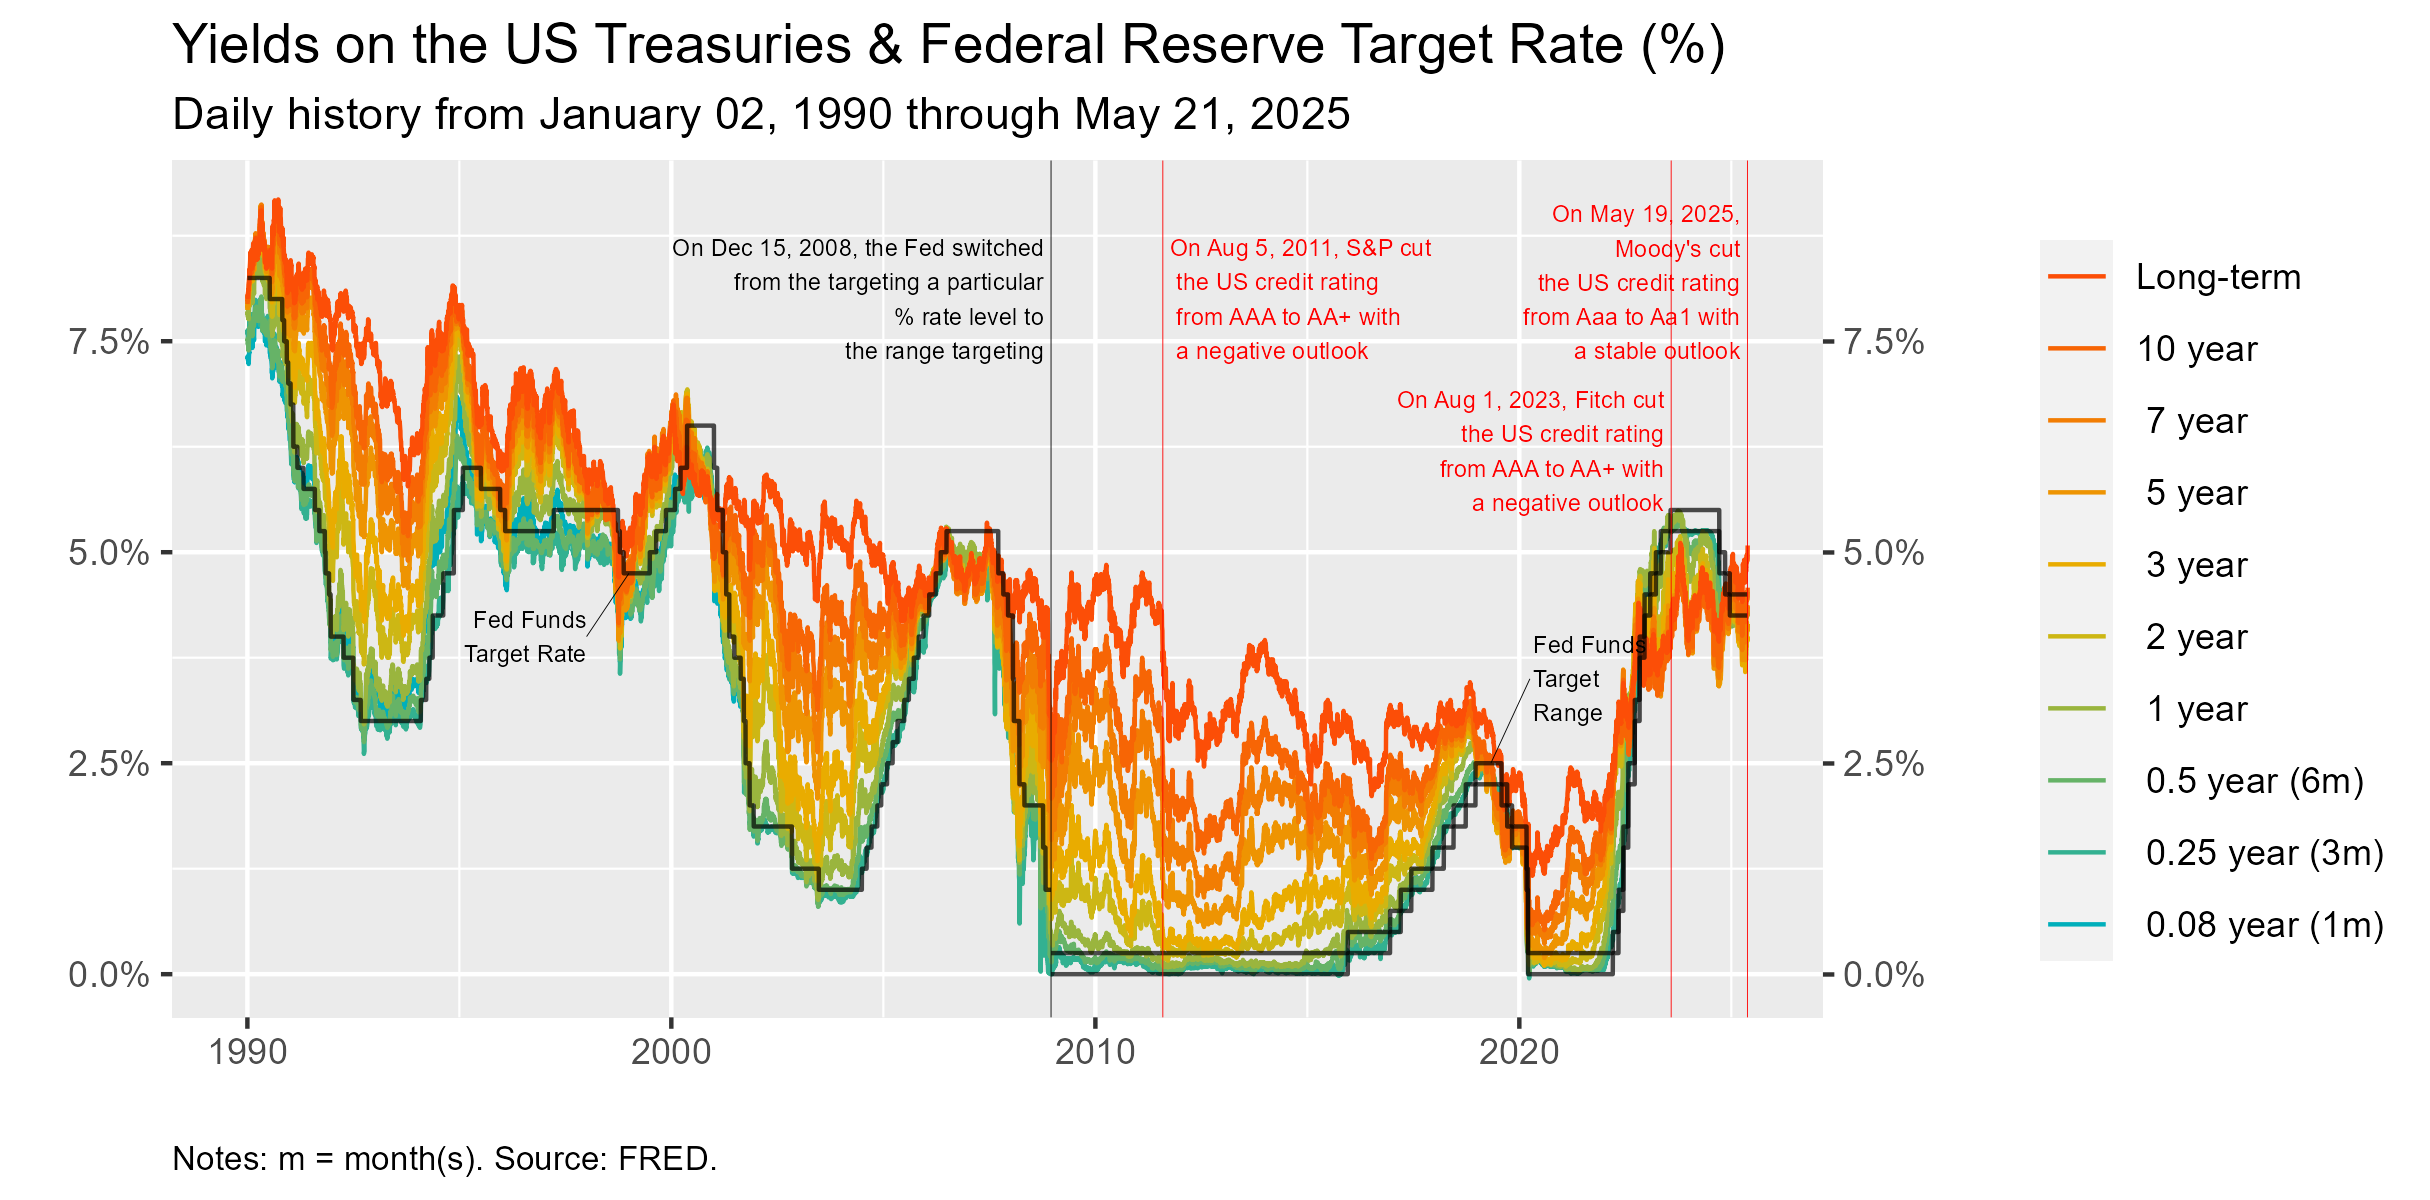
\includegraphics[width=1\linewidth]{Plots/Plot 3.png}
    \vspace{.2in}
    \caption*{Note: some notes. \par\vspace{.15in} Source: Federal Reserve System of the United States}
    \vspace{.2in}
    \label{fig:plot3}
\end{figure}

\lipsum[3]

\subsection{Some Second Title}\label{apx:B}

\subsubsection*{Some title}
\lipsum[4]

\begin{figure}[htbp]
    \vspace{.2in}
    % The figure's caption and notes lines are centered, 100% of page width 
    \captionsetup{width=1\linewidth,labelfont=bf}
    \caption{Example of a large plot, showing monthly data points, which is placed on a separate page in Appendix~\ref{apx:B}}
    \vspace{.2in}
    \centering
    % The plot is 100% of its width
    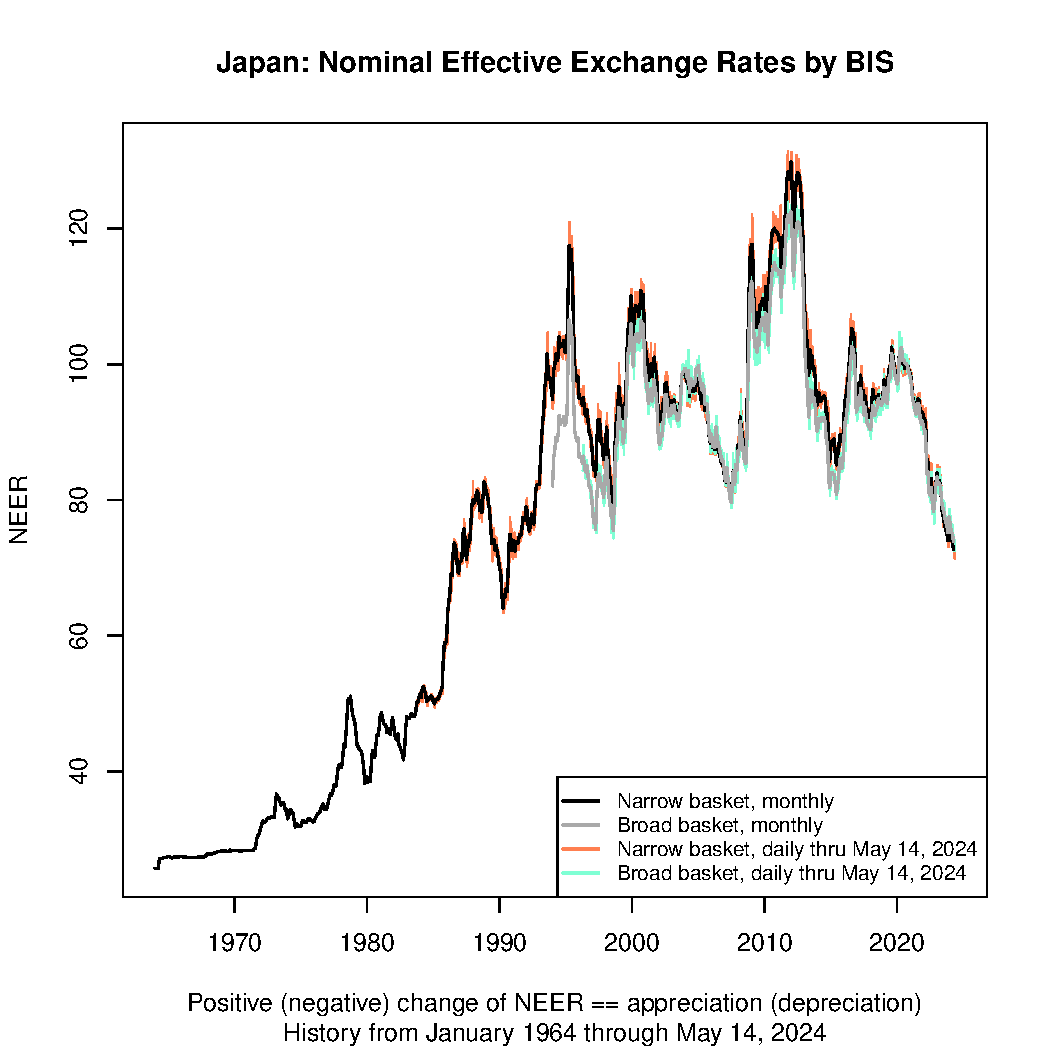
\includegraphics[width=1\linewidth]{Plots/Plot 2.pdf}
    \vspace{.2in}
    \caption*{Note: some notes. \par\vspace{.15in} Source: \ac{bis}, \url{https://www.bis.org/}}
    \vspace{.2in}
    \label{fig:plot2}
\end{figure}

\subsubsection*{Some title}
\lipsum[5]

\begin{sidewaysfigure}[htbp]
    \captionsetup{width=1\linewidth,labelfont=bf}
    \caption{Example of an elaborate, landscape \emph{TiKz} plot}
    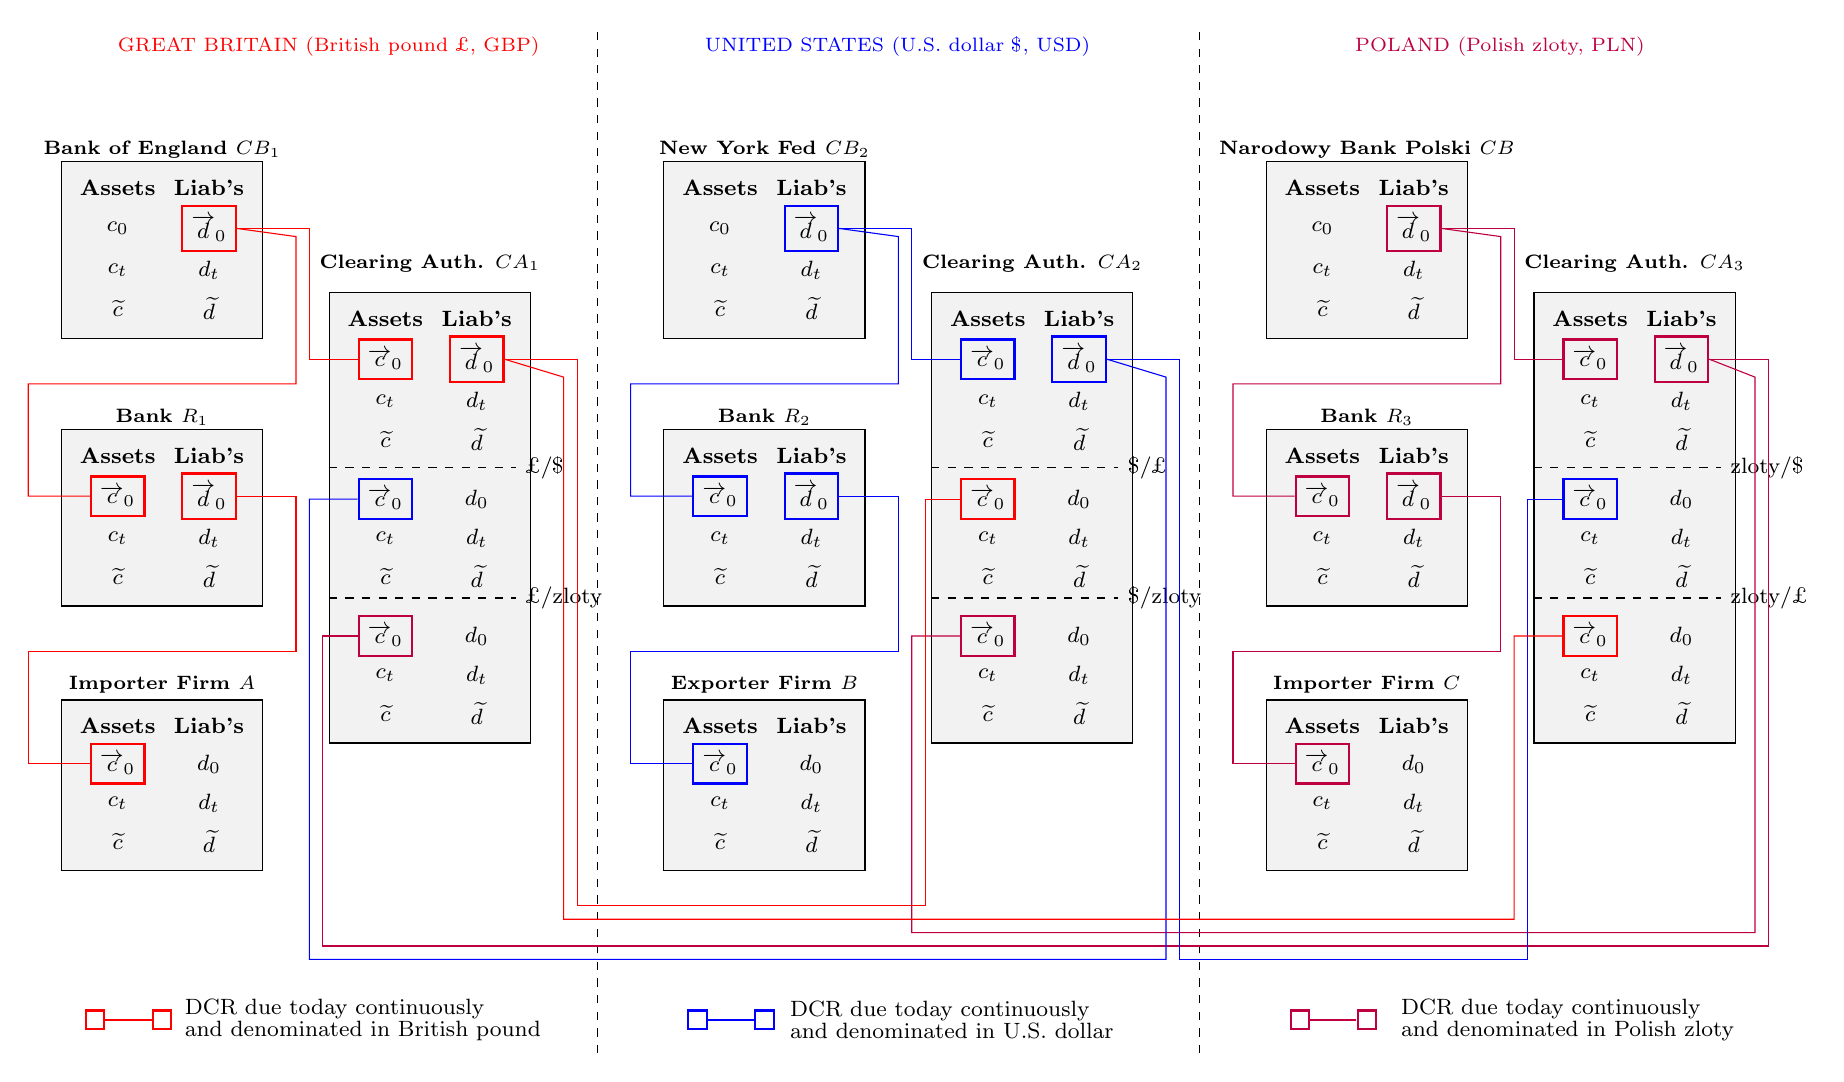
\begin{tikzpicture}[scale=.85]
    \draw[help lines,white] (0,0) grid (26,14);
    \draw[black,dashed] (8.5,-1) -- (8.5,14.25); 
    \draw[black,dashed] (17.5,-1) -- (17.5,14.25); 
    \node[red]  at (4.5,14) {\textsuperscript{\MakeUppercase{Great Britain} (British pound \pounds, GBP)}};
    \node[blue] at (13,14) {\textsuperscript{\MakeUppercase{United States} (U.S. dollar \$, USD)}};
    \node[purple] at (22,14) {\textsuperscript{\MakeUppercase{Poland} (Polish zloty, PLN)}};
  % US ====================================================
    % NY Fed ------------------------------------------------------------
        \node [matrix,fill=gray!10,draw=black,thin,font=\bf\fontsize{8}{8}\selectfont] (cb) at (11,11) {
            \node {Assets}; & \node {Liab's}; \\
            \node (CB_c0) {$c_0$}; & \node[rectangle,draw=blue,thick] (CB_d0)  {$\overrightarrow{d}_0$}; \\
            \node {$c_t$}; & \node {$d_t$}; \\
            \node {$\widetilde{c}$}; & \node {$\widetilde{d}$}; \\
            };
        \draw (cb)++(0,1.5) node[font=\bf\fontsize{7}{7}\selectfont]%
            {New York Fed $CB_2$};
    % Bank R1 ------------------------------------------------------------
        \node [matrix,fill=gray!10,draw=black,thin,font=\bf\fontsize{8}{8}\selectfont] (cb) at (11,7) {
            \node {Assets}; & \node {Liab's}; \\
            \node[rectangle,draw=blue,thick] (R1_c0) {$\overrightarrow{c}_0$}; & \node[rectangle,draw=blue,thick] (R1_d0) {$\overrightarrow{d}_0$}; \\
            \node {$c_t$}; & \node {$d_t$}; \\
            \node {$\widetilde{c}$}; & \node {$\widetilde{d}$}; \\
            };
        \draw (cb)++(0,1.5) node[font=\bf\fontsize{7}{7}\selectfont]%
            {Bank $R_2$};
    % Clearing Authority -------------------------------------------------
        \node [matrix,fill=gray!10,draw=black,thin,font=\bf\fontsize{8}{8}\selectfont] (CA2) at (15,7) {
            \node {Assets}; & \node {Liab's}; \\
            \node[rectangle,draw=blue,thick] (CA2_c0) {$\overrightarrow{c}_0$}; & \node[rectangle,draw=blue,thick] (CA2_d0) {$\overrightarrow{d}_0$}; \\
            \node {$c_t$}; & \node {$d_t$}; \\
            \node {$\widetilde{c}$}; & \node {$\widetilde{d}$}; \\
            \node {}; & \node {}; \\
            \node[rectangle,draw=red,thick] (CA2_fx1_c0) {$\overrightarrow{c}_0$}; & \node (CA2_fx_d0) {$d_0$}; \\
            \node {$c_t$}; & \node {$d_t$}; \\
            \node {$\widetilde{c}$}; & \node {$\widetilde{d}$}; \\
            \node {}; & \node {}; \\
            \node[rectangle,draw=purple,thick] (CA2_fx3_c0) {$\overrightarrow{c}_0$}; & \node (CA2_fx_d0) {$d_0$}; \\
            \node {$c_t$}; & \node {$d_t$}; \\
            \node {$\widetilde{c}$}; & \node {$\widetilde{d}$}; \\
            };
        \draw[dashed] (CA2.west)++(0,.75) -- +(2.8,0) node[at end ,right,font=\fontsize{8}{8}\selectfont] {\$/\pounds};
        \draw[dashed] (CA2.west)++(0,-1.2) -- +(2.8,0) node[at end ,right,font=\fontsize{8}{8}\selectfont] {\$/zloty};
        \draw (CA2)++(0,3.8) node[font=\bf\fontsize{7}{7}\selectfont]%
            {Clearing Auth. $CA_2$};
    % Exporter ----------------------------------------------
        \node [matrix,fill=gray!10,draw=black,thin,font=\bf\fontsize{8}{8}\selectfont] (cb) at (11,3) {
            \node {Assets}; & \node {Liab's}; \\
            \node[rectangle,draw=blue,thick] (B_c0) {$\overrightarrow{c}_0$}; & \node {$d_0$}; \\
            \node {$c_t$}; & \node {$d_t$}; \\
            \node {$\widetilde{c}$}; & \node {$\widetilde{d}$}; \\
            };
        \draw (cb)++(0,1.5) node[font=\bf\fontsize{7}{7}\selectfont]%
            {Exporter Firm $B$};
    \gettikzxy{(CB_d0)}{\ax}{\ay}; \gettikzxy{(R1_c0)}{\bx}{\by}
    \draw[blue] (CB_d0.east) -- (13,11.2) -- (13,9) -- (9,9) -- (9,\by) -- (R1_c0.west);
    \gettikzxy{(CB_d0)}{\ax}{\ay}; \gettikzxy{(CA2_c0)}{\bx}{\by}
    \draw[blue] (CB_d0.east) -- (13.2,\ay) -- (13.2,\by) -- (CA2_c0.west);
    \gettikzxy{(R1_d0)}{\ax}{\ay}; \gettikzxy{(B_c0)}{\bx}{\by}
    \draw[blue] (R1_d0.east) -- (13,\ay) -- (13,5) -- (9,5) -- (9,\by) -- (B_c0.west);
    \draw[blue,thick] (10,-.5) node(a)[draw] {} (11,-.5) node(b)[draw] {};
    \draw[blue,thick] (a) -- (b);
    \node[black,align=left,font=\fontsize{8}{8}\selectfont] at (13.8,-.5)%
        {DCR due today continuously\\and denominated in U.S. dollar};
    % MX ====================================================
    % BoE ----------------------------------------------------------
        \node [matrix,fill=gray!10,draw=black,thin,font=\bf\fontsize{8}{8}\selectfont] (cb) at (2,11) {
            \node {Assets}; & \node {Liab's}; \\
            \node (CB_c0) {$c_0$}; & \node[rectangle,draw=red,thick] (CB_d0)  {$\overrightarrow{d}_0$}; \\
            \node {$c_t$}; & \node {$d_t$}; \\
            \node {$\widetilde{c}$}; & \node {$\widetilde{d}$}; \\
            };
        \draw (cb)++(0,1.5) node[font=\bf\fontsize{7}{7}\selectfont]%
            {Bank of England $CB_1$};
    % Bank R2 ------------------------------------------------------------
        \node [matrix,fill=gray!10,draw=black,thin,font=\bf\fontsize{8}{8}\selectfont] (cb) at (2,7) {
            \node {Assets}; & \node {Liab's}; \\
            \node[rectangle,draw=red,thick] (R2_c0) {$\overrightarrow{c}_0$}; & \node[rectangle,draw=red,thick] (R2_d0) {$\overrightarrow{d}_0$}; \\
            \node {$c_t$}; & \node {$d_t$}; \\
            \node {$\widetilde{c}$}; & \node {$\widetilde{d}$}; \\
            };
        \draw (cb)++(0,1.5) node[font=\bf\fontsize{7}{7}\selectfont]%
            {Bank $R_1$};
    % Clearing Authority -------------------------------------------------
        \node [matrix,fill=gray!10,draw=black,thin,font=\bf\fontsize{8}{8}\selectfont] (CA1) at (6,7) {
            \node {Assets}; & \node {Liab's}; \\
            \node[rectangle,draw=red,thick] (CA1_c0) {$\overrightarrow{c}_0$}; & \node[rectangle,draw=red,thick] (CA1_d0) {$\overrightarrow{d}_0$}; \\
            \node {$c_t$}; & \node {$d_t$}; \\
            \node {$\widetilde{c}$}; & \node {$\widetilde{d}$}; \\
            \node {}; & \node {}; \\
            \node[rectangle,draw=blue,thick] (CA1_fx2_c0) {$\overrightarrow{c}_0$}; & \node (CA1_fx_d0) {$d_0$}; \\
            \node {$c_t$}; & \node {$d_t$}; \\
            \node {$\widetilde{c}$}; & \node {$\widetilde{d}$}; \\
            \node {}; & \node {}; \\
            \node[rectangle,draw=purple,thick] (CA1_fx3_c0) {$\overrightarrow{c}_0$}; & \node (CA1_fx_d0) {$d_0$}; \\
            \node {$c_t$}; & \node {$d_t$}; \\
            \node {$\widetilde{c}$}; & \node {$\widetilde{d}$}; \\
            };
        \draw[dashed] (CA1.west)++(0,.75) -- +(2.8,0) node[at end ,right,font=\fontsize{8}{8}\selectfont] {\pounds/\$};
        \draw[dashed] (CA1.west)++(0,-1.2) -- +(2.8,0) node[at end ,right,font=\fontsize{8}{8}\selectfont] {\pounds/zloty};
        \draw (CA1)++(0,3.8) node[font=\bf\fontsize{7}{7}\selectfont]%
            {Clearing Auth. $CA_1$};
    % Exporter ----------------------------------------------
        \node [matrix,fill=gray!10,draw=black,thin,font=\bf\fontsize{8}{8}\selectfont] (cb) at (2,3) {
            \node {Assets}; & \node {Liab's}; \\
            \node[rectangle,draw=red,thick] (A_c0) {$\overrightarrow{c}_0$}; & \node {$d_0$}; \\
            \node {$c_t$}; & \node {$d_t$}; \\
            \node {$\widetilde{c}$}; & \node {$\widetilde{d}$}; \\
            };
        \draw (cb)++(0,1.5) node[font=\bf\fontsize{7}{7}\selectfont]%
            {Importer Firm $A$};
    \gettikzxy{(CB_d0)}{\ax}{\ay}; \gettikzxy{(R2_c0)}{\bx}{\by}
    \draw[red] (CB_d0.east) -- (4,11.2) -- (4,9) -- (0,9) -- (0,\by) -- (R2_c0.west);
    \gettikzxy{(CB_d0)}{\ax}{\ay}; \gettikzxy{(CA1_c0)}{\bx}{\by}
    \draw[red] (CB_d0.east) -- (4.2,\ay) -- (4.2,\by) -- (CA1_c0.west);
    \gettikzxy{(R2_d0)}{\ax}{\ay}; \gettikzxy{(A_c0)}{\bx}{\by}
    \draw[red] (R2_d0.east) -- (4,\ay) -- (4,5) -- (0,5) -- (0,\by) -- (A_c0.west);
    \draw[red,thick] (1,-.5) node(a)[draw] {} (2,-.5) node(b)[draw] {};
    \draw[red,thick] (a) -- (b);
    \node[black,align=left,font=\fontsize{8}{8}\selectfont] at (5,-.5)%
        {DCR due today continuously\\and denominated in British pound};
    % PL ====================================================
    % Bank of Poland ----------------------------------------------------------
        \node [matrix,fill=gray!10,draw=black,thin,font=\bf\fontsize{8}{8}\selectfont] (cb) at (20,11) {
            \node {Assets}; & \node {Liab's}; \\
            \node (CB_c0) {$c_0$}; & \node[rectangle,draw=purple,thick] (CB_d0)  {$\overrightarrow{d}_0$}; \\
            \node {$c_t$}; & \node {$d_t$}; \\
            \node {$\widetilde{c}$}; & \node {$\widetilde{d}$}; \\
            };
        \draw (cb)++(0,1.5) node[font=\bf\fontsize{7}{7}\selectfont]%
            {Narodowy Bank Polski $CB$};
    % Bank R3 ------------------------------------------------------------
        \node [matrix,fill=gray!10,draw=black,thin,font=\bf\fontsize{8}{8}\selectfont] (cb) at (20,7) {
            \node {Assets}; & \node {Liab's}; \\
            \node[rectangle,draw=purple,thick] (R2_c0) {$\overrightarrow{c}_0$}; & \node[rectangle,draw=purple,thick] (R2_d0) {$\overrightarrow{d}_0$}; \\
            \node {$c_t$}; & \node {$d_t$}; \\
            \node {$\widetilde{c}$}; & \node {$\widetilde{d}$}; \\
            };
        \draw (cb)++(0,1.5) node[font=\bf\fontsize{7}{7}\selectfont]%
            {Bank $R_3$};
    % Clearing Authority -------------------------------------------------
        \node [matrix,fill=gray!10,draw=black,thin,font=\bf\fontsize{8}{8}\selectfont] (CA3) at (24,7) {
            \node {Assets}; & \node {Liab's}; \\
            \node[rectangle,draw=purple,thick] (CA3_c0) {$\overrightarrow{c}_0$}; & \node[rectangle,draw=purple,thick] (CA3_d0) {$\overrightarrow{d}_0$}; \\
            \node {$c_t$}; & \node {$d_t$}; \\
            \node {$\widetilde{c}$}; & \node {$\widetilde{d}$}; \\
            \node {}; & \node {}; \\
            \node[rectangle,draw=blue,thick] (CA3_fx2_c0) {$\overrightarrow{c}_0$}; & \node (CA3_fx_d0) {$d_0$}; \\
            \node {$c_t$}; & \node {$d_t$}; \\
            \node {$\widetilde{c}$}; & \node {$\widetilde{d}$}; \\
            \node {}; & \node {}; \\
            \node[rectangle,draw=red,thick] (CA3_fx1_c0) {$\overrightarrow{c}_0$}; & \node (CA3_fx_d0) {$d_0$}; \\
            \node {$c_t$}; & \node {$d_t$}; \\
            \node {$\widetilde{c}$}; & \node {$\widetilde{d}$}; \\
            };
        \draw[dashed] (CA3.west)++(0,.75) -- +(2.8,0) node[at end ,right,font=\fontsize{8}{8}\selectfont] {zloty/\$};
        \draw[dashed] (CA3.west)++(0,-1.2) -- +(2.8,0) node[at end ,right,font=\fontsize{8}{8}\selectfont] {zloty/\pounds};
        \draw (CA3)++(0,3.8) node[font=\bf\fontsize{7}{7}\selectfont]%
            {Clearing Auth. $CA_3$};
    % Exporter ----------------------------------------------
        \node [matrix,fill=gray!10,draw=black,thin,font=\bf\fontsize{8}{8}\selectfont] (cb) at (20,3) {
            \node {Assets}; & \node {Liab's}; \\
            \node[rectangle,draw=purple,thick] (A_c0) {$\overrightarrow{c}_0$}; & \node {$d_0$}; \\
            \node {$c_t$}; & \node {$d_t$}; \\
            \node {$\widetilde{c}$}; & \node {$\widetilde{d}$}; \\
            };
        \draw (cb)++(0,1.5) node[font=\bf\fontsize{7}{7}\selectfont]%
            {Importer Firm $C$};
    \gettikzxy{(CB_d0)}{\ax}{\ay}; \gettikzxy{(R2_c0)}{\bx}{\by}
    \draw[purple] (CB_d0.east) -- (22,11.2) -- (22,9) -- (18,9) -- (18,\by) -- (R2_c0.west);
    \gettikzxy{(CB_d0)}{\ax}{\ay}; \gettikzxy{(CA3_c0)}{\bx}{\by}
    \draw[purple] (CB_d0.east) -- (22.2,\ay) -- (22.2,\by) -- (CA3_c0.west);
    \gettikzxy{(R2_d0)}{\ax}{\ay}; \gettikzxy{(A_c0)}{\bx}{\by}
    \draw[purple] (R2_d0.east) -- (22,\ay) -- (22,5) -- (18,5) -- (18,\by) -- (A_c0.west);
    \draw[purple,thick] (19,-.5) node(a)[draw] {} (20,-.5) node(b)[draw] {};
    \draw[purple,thick] (a) -- (b);
    \node[black,align=left,font=\fontsize{8}{8}\selectfont] at (23,-.5)%
        {DCR due today continuously\\and denominated in Polish zloty};
    % ================================================================
    \gettikzxy{(CA1_fx3_c0)}{\ax}{\ay}; \gettikzxy{(CA3_d0)}{\bx}{\by}
    \draw[purple] (CA1_fx3_c0.west) -- (4.4,\ay) -- (4.4,.6) -- (26,.6) -- (26,\by) -- (CA3_d0.east);
    \gettikzxy{(CA2_fx3_c0)}{\ax}{\ay}; \gettikzxy{(CA3_d0)}{\bx}{\by}
    \draw[purple] (CA2_fx3_c0.west) -- (13.2,\ay) -- (13.2,.8) -- (25.8,.8) -- (25.8,9.1) -- (CA3_d0.east);
    \gettikzxy{(CA1_fx2_c0)}{\ax}{\ay}; \gettikzxy{(CA2_d0)}{\bx}{\by}
    \draw[blue] (CA1_fx2_c0.west) -- (4.2,\ay) -- (4.2,.4) -- (17,.4) -- (17,9.1) -- (CA2_d0.east);
    \gettikzxy{(CA3_fx2_c0)}{\ax}{\ay}; \gettikzxy{(CA2_d0)}{\bx}{\by}
    \draw[blue] (CA3_fx2_c0.west) -- (22.4,\ay) -- (22.4,.4) -- (17.2,.4) -- (17.2,\by) -- (CA2_d0.east);
    \gettikzxy{(CA3_fx1_c0)}{\ax}{\ay}; \gettikzxy{(CA1_d0)}{\bx}{\by}
    \draw[red] (CA3_fx1_c0.west) -- (22.2,\ay) -- (22.2,1) -- (8,1) -- (8,9.1) -- (CA1_d0.east);
    \gettikzxy{(CA2_fx1_c0)}{\ax}{\ay}; \gettikzxy{(CA1_d0)}{\bx}{\by}
    \draw[red] (CA2_fx1_c0.west) -- (13.4,\ay) -- (13.4,1.2) -- (8.2,1.2) -- (8.2,\by) -- (CA1_d0.east);
\end{tikzpicture}

    \caption*{Notes: some notes here. \par\vspace{.15in} Source: \url{https://github.com/valchyshen}}
    \label{fig:tikz2}
\end{sidewaysfigure}
\newpage \theendnotes % <------------ End-notes Section 
\newpage  
\addcontentsline{toc}{section}{\MakeUppercase{Footnotes}}
\newpage 
\printbibliography[title={\MakeUppercase{References}}] % <---- References
\addcontentsline{toc}{section}{\MakeUppercase{References}}
\newpage 
\section*{\MakeUppercase{Vita}}
\addcontentsline{toc}{section}{\MakeUppercase{Vita}}

% Place your VITA below instead of a UMKC short description below, in line 6

This last section of the T/D, VITA, is written in paragraph form, in third person, and is double-spaced. It is a type of biographical sketch, and it is different from a Curriculum Vitae. In the VITA, the date, place of birth, and schools attended are optional, and it is not recommended to include them. The bio should only include professional information, such as degrees previously earned, academic positions held, academic honors, and major research accomplishments or publications % <------ VITA Section

\end{document} % === END OF THE DOCUMENT ==================================